% !TeX root = booklet-02.tex
\clearpage
\subsection{وابستگی به دما}
\label{sec:temperature-dependence}
افزایش دما، هم حرکت حامل‌ها و هم ولتاژ آستانه را تغییر می‌دهد. برای
محاسبه جریان، باید این تغییرها را هم‌زمان وارد مدل کرد
\cite[بخش \secnum{۲.۴.۵}، صفحات ۸۵ و ۸۶]{weste}
\cite[اسلاید ۲۹]{nonideal}. در این بخش، \(T\) دمای مطلق، \(T_r\)
دمای مرجع و \(\mu\) همان \lr{Mobility} مورد استفاده در مدل جریان است.

\subsubsection*{دمای مطلق، توان منفی و کاهش \lr{Mobility}}
ارتباط دمای سلسیوس \(t_C\) با دمای مطلق به صورت زیر است.
\[
 T/\unit{\kelvin}=t_C/\unit{\degreeCelsius}+273.15.
\]
مثلاً \(\qty{300}{\kelvin}\) برابر \(\qty{26.85}{\degreeCelsius}\)
است. اختلاف دمای یک کلوین با اختلاف یک درجه سلسیوس برابر است.
در نسبت دماها باید مقدار کلوین را به کار برد. نسبت دماهای سلسیوس
معنای مورد نیاز رابطه \eqref{eq:temperature-mobility} را ندارد.

تقریب تجربی رابطه \secnum{۲.۵۱} کتاب چنین است
\begin{equation}
 \boxed{\mu(T)=\mu(T_r)\left(\frac{T}{T_r}\right)^{-k_\mu}}.
 \label{eq:temperature-mobility}
\end{equation}
ضریب \(k_\mu\) بی‌بعد است و مرجع مقدار معمول آن را حدود \(1.5\)
می‌گیرد. هر دو طرف رابطه واحد \lr{Mobility} دارند. توان منفی یعنی
\(x^{-a}=1/x^a\). بنابراین، برای \(T>T_r\) و \(k_\mu>0\)، نسبت
\(\mu(T)/\mu(T_r)\) از یک کوچک‌تر می‌شود. تفسیر فیزیکی آن کاهش
حرکت‌پذیری حامل‌ها در اثر افزایش پراکندگی با گرم‌شدن شبکه است.

برای نمونه، با \(T_r=\qty{300}{\kelvin}\)،
\(T=\qty{400}{\kelvin}\) و \(k_\mu=1.5\)، داریم
\begin{equation}
 \frac{\mu(400)}{\mu(300)}
 =\left(\frac{4}{3}\right)^{-3/2}
 =\frac{1}{(4/3)\sqrt{4/3}}\approx0.6495.
 \label{eq:temperature-mobility-example}
\end{equation}
در این تقریب، \lr{Mobility} حدود \num{35.05} درصد کاهش یافته است.
عددهای داخل آرگومان \(\mu\) در این مثال برحسب کلوین‌اند.
با ثابت‌گرفتن \(C_{\mathrm{ox}}\) و هندسه، ضریب
\(\beta(T)=\mu(T)C_{\mathrm{ox}}W/L\) نیز همین نسبت را دارد.

\subsubsection*{آستانه و سرعت اشباع}
تقریب رابطه \secnum{۲.۵۲} کتاب برای آستانه \lr{nMOS} برابر است با
\begin{equation}
 \boxed{V_t(T)=V_t(T_r)-k_{vt}(T-T_r)}.
 \label{eq:temperature-threshold}
\end{equation}
ضریب مثبت \(k_{vt}\) واحد \(\unit{\volt\per\kelvin}\) دارد و مقدار
معمول آن در مرجع حدود \(\qty{1}{\milli\volt\per\kelvin}\) تا
\(\qty{2}{\milli\volt\per\kelvin}\) است. حاصل‌ضرب آن در اختلاف
دما یک ولتاژ است. برای \lr{pMOS}، همین نوع تقریب را بر بزرگی آستانه
\(V_{TP}=|V_{tp}|\) اعمال می‌کنیم. کاهش بزرگی آستانه منفی، مقدار
علامت‌دار \(V_{tp}\) را به صفر نزدیک می‌کند.

اگر \(V_t(300)=\qty{0.4}{\volt}\) و
\(k_{vt}=\qty{1}{\milli\volt\per\kelvin}\) فرض شوند، افزایش دما
به اندازه \(\qty{100}{\kelvin}\)، آستانه را
\(\qty{0.1}{\volt}\) کاهش می‌دهد و
\(V_t(400)=\qty{0.3}{\volt}\) می‌شود. در گیت ثابت، این تغییر،
اضافه‌ولتاژ \(V_{GS}-V_t\) را افزایش می‌دهد و جریان روشن را تقویت
می‌کند. در همان زمان، کاهش \lr{Mobility} جریان را تضعیف می‌کند.

سرعت اشباع \(v_{\mathrm{sat}}\) هم با افزایش دما کاهش می‌یابد.
کتاب برای افزایش دما از \(\qty{300}{\kelvin}\) به
\(\qty{400}{\kelvin}\)، کاهش حدود ۲۰ درصد را بیان می‌کند
\cite[صفحه ۸۵]{weste}. این اعداد پارامترهای تقریبی وابسته به فناوری‌اند.
در مدل میدان قوی، تغییر \(\mu\) باید در \(\beta\) و تغییر
\(v_{\mathrm{sat}}/\mu\) باید در \(E_c\) و \(V_c\) اعمال شود.

\subsubsection*{مثال آموزشی رقابت دو اثر در جریان روشن}
برای جداکردن نقش آستانه و \lr{Mobility}، از مدل مربعی اشباع استفاده
می‌کنیم. فرض‌های آموزشی عبارت‌اند از هندسه و
\(C_{\mathrm{ox}}\) ثابت، \(V_{SB}=0\)، صرف‌نظر از \lr{CLM} و
\lr{DIBL} و محدودیت سرعت، و مقادیر
\(T_r=\qty{300}{\kelvin}\)، \(k_\mu=1.5\)،
\(V_t(T_r)=\qty{0.4}{\volt}\)،
\(k_{vt}=\qty{0.001}{\volt\per\kelvin}\) و
\(\beta_r=\qty{200}{\micro\ampere\per\volt\squared}\).
در بایاس روشن \(V_{GS}=V_{DS}=V_{DD}\)، جای‌گذاری روابط دما می‌دهد
\begin{equation}
 I_{\mathrm{on}}(T)=\frac{\beta_r}{2}
 \left(\frac{T}{T_r}\right)^{-k_\mu}
 [V_{DD}-V_t(T_r)+k_{vt}(T-T_r)]^2.
 \label{eq:temperature-on-current}
\end{equation}
این رابطه برای \(V_{DD}>V_t(T)\) و ناحیه اشباع مدل به کار می‌رود.
چون در این مثال \(V_t(T)>0\) است، شرط
\(V_{DS}=V_{DD}\ge V_{DD}-V_t(T)\) برقرار می‌ماند.

با تعریف \(A_r=V_{DD}-V_t(T_r)\)، تقسیم جریان‌ها مراحل محاسبه را
آشکار می‌کند
\begin{equation}
 \frac{I_{\mathrm{on}}(T)}{I_{\mathrm{on}}(T_r)}
 =\left(\frac{T}{T_r}\right)^{-k_\mu}
 \left[1+\frac{k_{vt}(T-T_r)}{A_r}\right]^2.
 \label{eq:temperature-current-ratio}
\end{equation}
عامل نخست در دمای بالاتر کمتر از یک است. عامل دوم بزرگ‌تر از یک
می‌شود و برای \(A_r\) کوچک، اثر نسبی قوی‌تری دارد.
جدول \ref{tab:temperature-on-results} دو حالت را نشان می‌دهد.
\begin{table}[!htbp]
\centering
\small
\caption{جریان روشن در مثال آموزشی دما با مدل مربعی.}
\label{tab:temperature-on-results}
\begin{tabular}{ccccc}
\toprule
\(V_{DD}\)، \(\unit{\volt}\) & \(A_r\)، \(\unit{\volt}\) &
\(I(300)\)، \(\unit{\micro\ampere}\) &
\(I(400)\)، \(\unit{\micro\ampere}\) & \(I(400)/I(300)\)\\
\midrule
\num{1.2} & \num{0.8} & \num{64.00} & \num{52.61} & \num{0.8220}\\
\num{0.6} & \num{0.2} & \num{4.000} & \num{5.846} & \num{1.461}\\
\bottomrule
\end{tabular}
\end{table}
برای ردیف نخست، محاسبه نسبت برابر
\(0.6495(0.9/0.8)^2\) و برای ردیف دوم برابر
\(0.6495(0.3/0.2)^2\) است. در تغذیه بالاتر، کاهش
\lr{Mobility} غالب شده است. در تغذیه پایین‌تر، افزایش نسبی
اضافه‌ولتاژ گیت، جریان را افزایش داده است. شکل
\ref{fig:temperature-on-ratio} همین مدل را در بازه دما رسم می‌کند.
\begin{figure}[!htbp]
\centering
\begin{latin}
\PersianMathDigits
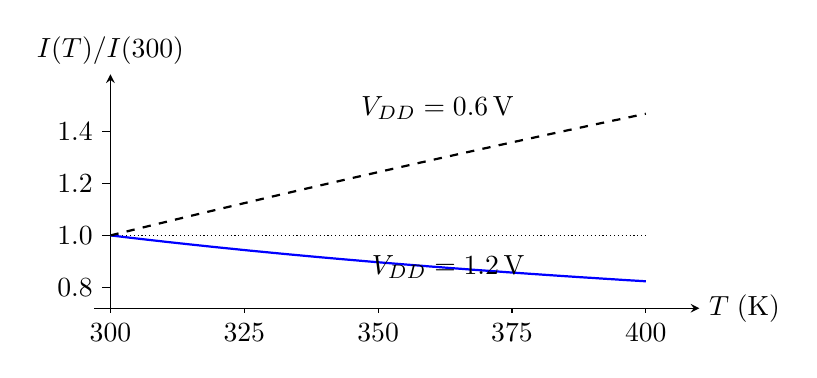
\begin{tikzpicture}[x=0.068cm,y=3.3cm,>=stealth]
\draw[->] (-3,0.72)--(110,0.72) node[right] {\(T\;(\mathrm{K})\)};
\draw[->] (0,0.72)--(0,1.62) node[above] {\(I(T)/I(300)\)};
\foreach \x/\t in {0/300,25/325,50/350,75/375,100/400}
 {\draw (\x,0.72)--(\x,0.70) node[below] {\(\t\)};}
\foreach \y in {0.8,1.0,1.2,1.4}
 {\draw (0,\y)--(-1.5,\y) node[left] {\(\y\)};}
\draw[densely dotted] (0,1)--(100,1);
\draw[thick,blue,domain=0:100,samples=70]
 plot (\x,{pow((300+\x)/300,-1.5)*pow((0.8+0.001*\x)/0.8,2)});
\draw[thick,dashed,domain=0:100,samples=70]
 plot (\x,{pow((300+\x)/300,-1.5)*pow((0.2+0.001*\x)/0.2,2)});
\node[anchor=west] at (47,0.88) {\(V_{DD}=1.2\,\mathrm{V}\)};
\node[anchor=west] at (45,1.49) {\(V_{DD}=0.6\,\mathrm{V}\)};
\end{tikzpicture}
\end{latin}
\caption{تغییر جریان نرمال‌شده برای پارامترهای فرضی مثال دما.
منحنی‌ها از رابطه \eqref{eq:temperature-current-ratio} محاسبه شده‌اند.}
\label{fig:temperature-on-ratio}
\end{figure}

\subsubsection*{معنای ضریب دمایی و استخراج شرط تغییر علامت}
مشتق \(\mathrm{d}I/\mathrm{d}T\)، نرخ تغییر جریان با تغییر کوچک
دماست. برای درک سهم عامل‌ها، می‌توان ابتدا تغییر نسبی را نوشت.
در مدل \eqref{eq:temperature-on-current}، جریان با \(\beta A^2\)
متناسب است که \(A(T)=V_{DD}-V_t(T)>0\) است. برای تغییر کوچک دما،
تغییر نسبی حاصل‌ضرب تقریباً برابر جمع تغییرهای نسبی عامل‌ها می‌شود
\begin{equation}
 \frac{\Delta I}{I}\approx
 \frac{\Delta\beta}{\beta}+2\frac{\Delta A}{A}.
 \label{eq:temperature-fractional-change}
\end{equation}
ضریب دو از مربع \(A\) می‌آید. مشتق دقیق همین بیان، با
\(\beta\propto T^{-k_\mu}\) و
\(\mathrm{d}A/\mathrm{d}T=k_{vt}\)، برابر است با
\begin{equation}
 \frac{1}{I}\frac{\mathrm{d}I}{\mathrm{d}T}
 =-\frac{k_\mu}{T}+\frac{2k_{vt}}{V_{DD}-V_t(T)}.
 \label{eq:temperature-coefficient}
\end{equation}
هر دو جمله واحد \(\unit{\per\kelvin}\) دارند. ضریب مثبت یعنی افزایش
جریان با گرم‌شدن در همسایگی همان نقطه. با صفرقراردادن طرف راست،
شرط توازن محلی به دست می‌آید
\begin{equation}
 V_{DD}-V_t(T)=\frac{2k_{vt}T}{k_\mu}.
 \label{eq:temperature-crossover}
\end{equation}
در \(\qty{300}{\kelvin}\) و با پارامترهای مثال، طرف راست
\(\qty{0.4}{\volt}\) است و توازن محلی در
\(V_{DD}=\qty{0.8}{\volt}\) رخ می‌دهد. این شرط، شیب جریان در یک
دمای مشخص را صفر می‌کند. برابری جریان در دو دمای با فاصله زیاد
باید مستقیماً از \eqref{eq:temperature-current-ratio} حل شود.

کتاب، رفتار معمول جریان روشن را در تغذیه بالا کاهشی توصیف می‌کند و
برای تغذیه پایین، افزایش جریان با دما را نیز مطرح می‌کند. بازه
تقریبی \(\qty{0.7}{\volt}\) تا \(\qty{1.1}{\volt}\) در متن کتاب به
نمونه‌های فناوری آن مرجع مربوط است. شکل‌های \secnum{۲.۲۳} و
\secnum{۲.۲۴} همان صفحه، تغییر شکل منحنی و کاهش معمول جریان روشن
را نمایش می‌دهند \cite[صفحه ۸۵]{weste}. تعیین نقطه تغییر علامت در
یک فناوری مشخص به مدل کامل همان فناوری نیاز دارد.

\subsubsection*{مثال آموزشی تغییر نشتی مطلق با دما}
در تمرین \secnum{۲.۱۰}، دو آستانه متفاوت در یک دمای مشترک مقایسه می‌شوند.
برای مقایسه دو دما، عامل پیش‌ضرب و ولتاژ حرارتی هم تغییر می‌کنند.
فرض کنید مدل \eqref{eq:leakage-subthreshold-model} با
\(V_{GS}=V_{SB}=0\)، \(V_{DS}=\qty{1}{\volt}\)، \(\eta=0\)،
\(n=1.4\) و همان \(\beta(T)\) و \(V_t(T)\) مثال دما به کار رود.
در این مدل آموزشی، \(n\)، هندسه و \(C_{\mathrm{ox}}\) ثابت‌اند.
اگر \(v_{T,i}=kT_i/q\) و
\(F_i=1-\exp(-V_{DS}/v_{T,i})\) باشند، تقسیم دو جریان می‌دهد
\begin{equation}
 \frac{I_2}{I_1}=
 \left(\frac{T_2}{T_1}\right)^{2-k_\mu}
 \exp\!\left[\frac{V_t(T_1)}{nv_{T,1}}
             -\frac{V_t(T_2)}{nv_{T,2}}\right]\frac{F_2}{F_1}.
 \label{eq:temperature-leakage-ratio}
\end{equation}
توان \(2-k_\mu\) از حاصل‌ضرب
\(\beta\propto T^{-k_\mu}\) و \(v_T^2\propto T^2\) در
\eqref{eq:leakage-current-prefactor} به دست آمده است.
ثابت تجربی \(e^{1.8}\) در نسبت حذف می‌شود.
با \(k/q\approx\qty{8.61733e-5}{\volt\per\kelvin}\)،
\(v_{T,1}\approx\qty{25.852}{\milli\volt}\) و
\(v_{T,2}\approx\qty{34.469}{\milli\volt}\) هستند.
در هر دو دما، \(V_{DS}/v_T>29\) و عامل \(F\) با دقت خوبی یک است.
جای‌گذاری \(V_t(300)=\qty{0.4}{\volt}\) و
\(V_t(400)=\qty{0.3}{\volt}\) نتیجه می‌دهد
\begin{equation}
 I_1\approx\qty{12.82}{\pico\ampere},\qquad
 I_2\approx\qty{1.864}{\nano\ampere},\qquad
 \frac{I_2}{I_1}\approx145.3.
 \label{eq:temperature-leakage-example}
\end{equation}
هر دو بایاس گیت زیر آستانه‌اند. رشد شدید در این مثال از تغییر عامل
نمایی ناشی می‌شود. مقدار واقعی رشد به پارامترها و بایاس وابسته است.
کتاب رشد شدید نشتی زیرآستانه، رشد آهسته‌تر \lr{BTBT} و وابستگی کم
نشتی گیت به دما را در محدوده بحث خود بیان می‌کند
\cite[صفحه ۸۵]{weste}. توان نشتی هر منبع از جریان همان منبع و
ولتاژ آن به دست می‌آید.

\subsubsection*{خنک‌کاری و سازگاری مدل میدان بحرانی}
کاهش دما معمولاً \lr{Mobility} را بیشتر و نشتی زیرآستانه را کمتر
می‌کند. مرجع، دفع گرما با همرفت، فن و \lr{Heat Sink} و روش‌های
قوی‌تر مانند خنک‌کاری آبی، سردکننده لایه‌نازک و نیتروژن مایع را
مطرح می‌کند. کاهش نشتی می‌تواند به انتخاب آستانه کمتر کمک کند.
متن همچنین افزایش پهنای ناحیه تخلیه و کاهش ظرفیت پیوند را در بحث
عملکرد دمای پایین بیان می‌کند \cite[صفحه ۸۶]{weste}.
این نتایج با فرض‌های بایاس و فناوری همان بحث تفسیر می‌شوند.

برای جهت تغییر \(E_c\)، رابطه \eqref{eq:critical-field} باید با هر
دو پارامتر بررسی شود. با تقریب‌های عددی همین بخش، داریم
\begin{equation}
 \frac{E_c(400)}{E_c(300)}
 =\frac{v_{\mathrm{sat}}(400)/v_{\mathrm{sat}}(300)}
        {\mu(400)/\mu(300)}
 \approx\frac{0.8}{0.6495}\approx1.232.
 \label{eq:temperature-critical-field}
\end{equation}
پس ترکیب این تقریب‌ها، میدان بحرانی بزرگ‌تر را در دمای بالاتر
می‌دهد. عبارت کیفی صفحه ۸۶ درباره وقوع اشباع سرعت در میدان‌های
بالاتر هنگام خنک‌کاری، با این انتخاب هم‌زمان پارامترها سازگار
نیست. در محاسبه این جزوه، جهت تغییر از نسبت
\(2v_{\mathrm{sat}}/\mu\) و داده‌های مدل تعیین می‌شود.

مرجع استفاده کوتاه‌مدت از اسپری سردکننده و دمنده هوای گرم را برای
تشخیص حساسیت دمایی مدار نیز بیان می‌کند و امکان آسیب ناشی از تغییر
ناگهانی دما به تراشه یا بسته‌بندی را یادآور می‌شود
\cite[صفحه ۸۶]{weste}. این توصیف، بخشی از محتوای مرجع است.

\clearpage
\subsection{وابستگی به هندسه}
\label{sec:geometry-dependence}
ابعاد ترسیم‌شده در \lr{Layout} با ابعاد مؤثر کانال تفاوت دارند.
کتاب و اسلایدها این تفاوت را با دو نوع اصلاح مدل می‌کنند
\cite[بخش \secnum{۲.۴.۶}، صفحه ۸۶]{weste}
\cite[اسلایدهای ۳۵ و ۳۶]{nonideal}. نمادهای
\(L_{\mathrm{drawn}},W_{\mathrm{drawn}}\) طول و عرض ترسیم‌شده‌اند.
اصلاح‌های علامت‌دار \(X_L,X_W\) تغییر ناشی از ساخت ماسک و فرایند
ساخت را نمایش می‌دهند. مثلاً \lr{Overetch} می‌تواند طول گیت را
کوتاه کند و \(X_L<0\) بدهد. پارامتر \(L_D\) سهم نفوذ جانبی از هر
طرف و \(W_D\) اصلاح کاهش عرض از هر لبه است.

\subsubsection*{استخراج ابعاد مؤثر و معنای ضریب دو}
پس از اصلاح ساخت، طول هندسی گیت
\(L_g=L_{\mathrm{drawn}}+X_L\) است. ناحیه‌های سورس و درین هر کدام
به اندازه \(L_D\) زیر گیت پیشروی می‌کنند. فاصله مؤثر عبور حامل‌ها
با کم‌کردن هر دو سهم به دست می‌آید. رابطه عرض نیز دو لبه دارد.
در نتیجه، رابطه \secnum{۲.۵۳} کتاب چنین نوشته می‌شود
\begin{align}
 L_{\mathrm{eff}}&=L_{\mathrm{drawn}}+X_L-2L_D,
 \label{eq:geometry-effective-length}\\
 W_{\mathrm{eff}}&=W_{\mathrm{drawn}}+X_W-2W_D.
 \label{eq:geometry-effective-width}
\end{align}
همه جمله‌ها واحد طول دارند. مقدارهای حاصل باید مثبت و در دامنه
اعتبار مدل فرایند باشند. شکل \ref{fig:geometry-length} سهم دو لبه
را به‌صورت شماتیک نمایش می‌دهد.
\begin{figure}[!htbp]
\centering
\begin{latin}
\PersianMathDigits
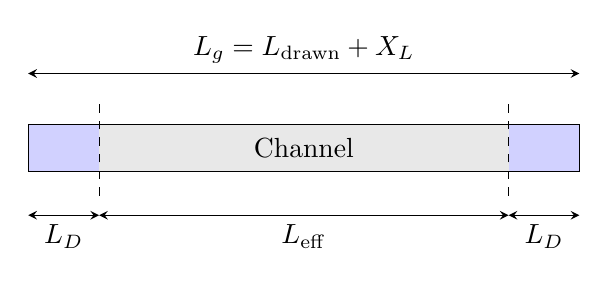
\begin{tikzpicture}[x=1cm,y=1cm,>=stealth]
\fill[gray!18] (0,0) rectangle (7,0.6);
\fill[blue!18] (0,0) rectangle (0.9,0.6);
\fill[blue!18] (6.1,0) rectangle (7,0.6);
\draw (0,0) rectangle (7,0.6);
\draw[dashed] (0.9,-0.3)--(0.9,0.9);
\draw[dashed] (6.1,-0.3)--(6.1,0.9);
\draw[<->] (0,1.25)--(7,1.25)
 node[midway,above] {\(L_g=L_{\mathrm{drawn}}+X_L\)};
\draw[<->] (0,-0.55)--(0.9,-0.55) node[midway,below] {\(L_D\)};
\draw[<->] (0.9,-0.55)--(6.1,-0.55)
 node[midway,below] {\(L_{\mathrm{eff}}\)};
\draw[<->] (6.1,-0.55)--(7,-0.55) node[midway,below] {\(L_D\)};
\node at (3.5,0.3) {Channel};
\end{tikzpicture}
\end{latin}
\caption{طرح آموزشی سهم نفوذ جانبی از دو سمت در طول مؤثر.
ابعاد شکل مقیاس فیزیکی ندارند.}
\label{fig:geometry-length}
\end{figure}

در بخش \ref{sec:clm}، نماد \(L_d\) با زیرنویس کوچک برای پیشروی
ناحیه تخلیه سمت درین در اثر بایاس به کار رفت. نماد \(L_D\) در این
بخش به نفوذ جانبی ناشی از ساخت مربوط است. هنگام ترکیب مدل‌ها، مرجع
طول و اصلاح بایاس را مشخص کنید تا یک کاهش طول دوبار وارد نشود.
در مدل \lr{CLM} ساده، \(\lambda\) اثر بایاس را در ضریب جریان
نمایش می‌دهد.

\subsubsection*{مثال آموزشی دوبرابرکردن طول و عرض ترسیم‌شده}
فرض کنید تمام ابعاد زیر برحسب نانومتر باشند و
\(X_L=X_W=-\qty{4}{\nano\metre}\)،
\(L_D=W_D=\qty{3}{\nano\metre}\).
برای افزاره مبنا با
\(L_{\mathrm{drawn}}=\qty{60}{\nano\metre}\) و
\(W_{\mathrm{drawn}}=\qty{120}{\nano\metre}\)، داریم
\[
 \begin{aligned}
 L_{\mathrm{eff}}&=60-4-2(3)=\qty{50}{\nano\metre},\\
 W_{\mathrm{eff}}&=120-4-2(3)=\qty{110}{\nano\metre}.
 \end{aligned}
\]
دوبرابرکردن طول ترسیم‌شده، طول مؤثر را به
\(120-4-6=\qty{110}{\nano\metre}\) می‌رساند. نسبت طول‌های مؤثر
\(110/50=2.2\) است. به همین ترتیب، دوبرابرکردن عرض ترسیم‌شده،
عرض مؤثر را \(\qty{230}{\nano\metre}\) می‌کند و نسبت عرض‌ها
\(230/110\approx2.091\) می‌شود.

برای محاسبه اثر هندسه به‌تنهایی، به‌طور آموزشی
\(k'=\mu C_{\mathrm{ox}}=\qty{200}{\micro\ampere\per\volt\squared}\)
و \(C_{\mathrm{ox}}=\qty{20}{\femto\farad\per\micro\metre\squared}\)
را ثابت فرض می‌کنیم. در تقریب مساحت مستطیلی کانال،
\begin{equation}
 \beta=k'\frac{W_{\mathrm{eff}}}{L_{\mathrm{eff}}},\qquad
 C_0=C_{\mathrm{ox}}W_{\mathrm{eff}}L_{\mathrm{eff}}.
 \label{eq:geometry-beta-capacitance}
\end{equation}
کمیت \(C_0\) مقیاس ظرفیت ذاتی گیت است. ظرفیت مؤثر هر پایانه به
ناحیه کاری و تقسیم بار وابسته است و ظرفیت‌های هم‌پوشانی و پیوند
نیز جداگانه مطرح‌اند. جدول \ref{tab:geometry-results} این محاسبه
هندسی را نشان می‌دهد.
\begin{table}[!htbp]
\centering
\small
\caption{نتایج هندسه فرضی با پارامترهای ماده ثابت.
طول‌ها برحسب \(\unit{\nano\metre}\) هستند.}
\label{tab:geometry-results}
\begin{tabularx}{\linewidth}{>{\raggedleft\arraybackslash}Xcccc}
\toprule
حالت & \(L_{\mathrm{eff}}\) & \(W_{\mathrm{eff}}\) &
\(\beta\)، \(\unit{\micro\ampere\per\volt\squared}\) &
\(C_0\)، \(\unit{\femto\farad}\)\\
\midrule
مبنا & \num{50} & \num{110} & \num{440} & \num{0.110}\\
طول ترسیم‌شده دوبرابر & \num{110} & \num{110} & \num{200} & \num{0.242}\\
عرض ترسیم‌شده دوبرابر & \num{50} & \num{230} & \num{920} & \num{0.230}\\
\bottomrule
\end{tabularx}
\end{table}
برای نمونه، \(\qty{50}{\nano\metre}=\qty{0.05}{\micro\metre}\)
و \(\qty{110}{\nano\metre}=\qty{0.11}{\micro\metre}\)، پس
مساحت مبنا \(\qty{0.0055}{\micro\metre\squared}\) است و
\(C_0=20(0.0055)=\qty{0.11}{\femto\farad}\) می‌شود.
در مدل مربعی با آستانه و بایاس ثابت، نسبت جریان برای تغییر طول
\(200/440\approx0.4545\) و برای تغییر عرض
\(920/440\approx2.091\) است.

در افزاره واقعی، هندسه می‌تواند آستانه را از راه اثر کانال کوتاه
و باریک نیز تغییر دهد. همچنین تغییر طول بر \lr{CLM} و
\lr{Velocity Saturation} اثر می‌گذارد. بنابراین، برای پیش‌بینی
جریان باید همه پارامترهای وابسته به هندسه را به‌روز کرد.
اسلاید ۳۶ افزایش آستانه و کاهش \lr{CLM} در کانال بلندتر را برای
روندهای مورد بحث دوره بیان می‌کند. نتیجه ساده \(I\propto1/L\)
به فرض ثابت‌بودن پارامترهای دیگر وابسته است
\cite[صفحه ۸۶]{weste}\cite[اسلاید ۳۶]{nonideal}.

\subsubsection*{هندسه یکسان و \lr{Matching}}
وقتی برابری یا نسبت دقیق جریان مهم است، کتاب استفاده از افزاره‌های
با طول و عرض یکسان را پیشنهاد می‌کند. برای نسبت‌های صحیح می‌توان
چند افزاره واحد یکسان را موازی کرد. مثلاً سه واحد موازی با بایاس‌های
پایانه‌ای یکسان، در مدل افزاره‌های یکسان سه برابر یک واحد جریان دارند.
هر واحد، همان اصلاح هندسی و آستانه واحد مبنا را تجربه می‌کند.

جهت‌گیری و محیط اطراف نیز بر ساخت اثر دارند. مرجع برای نمونه‌های
فرایندی کوچک‌تر از \(\qty{0.25}{\micro\metre}\)، اهمیت جهت‌گیری را
ذکر می‌کند. مقدار \lr{Polysilicon} مجاور می‌تواند سرعت حکاکی را
عوض کند. جهت‌گیری مشترک و \lr{Dummy Polysilicon} به یکنواختی محیط
کمک می‌کنند. چیدمان \lr{Interdigitated} یعنی درهم‌گذاری واحدهای
دو گروه، مانند ترتیب \lr{ABAB}، تا گروه‌ها محیط مکانی مشابه‌تری
ببینند. کتاب استفاده از آن را در صورت امکان مطرح می‌کند
\cite[صفحات ۸۶ و ۸۷]{weste}. انتخاب چیدمان واقعی تابع قواعد همان
فرایند و نوع خطای مورد کنترل است.

\subsubsection*{مکمل اسلایدها درباره \lr{PVT} و \lr{Process Corners}}
\label{sec:pvt-supplement}
اسلایدهای ۳۱ تا ۳۴، تغییر پارامترهای ساخت، تغذیه و دما را نیز
معرفی می‌کنند \cite{nonideal}. عبارت \lr{PVT} مخفف
\lr{Process, Voltage, Temperature} است. طول مؤثر، آستانه و ضخامت
عایق، مقادیر قطعی یکسان برای همه تراشه‌ها ندارند. تغذیه و دما نیز
در زمان و مکان تغییر می‌کنند. \lr{Corner} مجموعه‌ای مشخص از شرایط
مدل برای بررسی رفتار مدار است.

در قرارداد اسلایدها، \lr{T} به معنی \lr{Typical}، \lr{F} به معنی
\lr{Fast} و \lr{S} به معنی \lr{Slow} است. در مثال فرایندی اسلاید
۳۱، طول کوتاه‌تر، آستانه کمتر و عایق نازک‌تر به جریان قوی‌تر و
رفتار سریع‌تر کمک می‌کنند. پارامترهای \lr{nMOS} و \lr{pMOS} کاملاً
مستقل نیستند. دو حرف \lr{FS} یعنی \lr{nMOS} سریع و \lr{pMOS} کند،
و \lr{SF} حالت معکوس آن است. \lr{TT}، \lr{FF} و \lr{SS} نیز
به‌ترتیب حالت معمول و دو حالت هم‌جهت را نمایش می‌دهند.

اسلاید ۳۳ برای توصیف کامل‌تر، چهار حرف را به ترتیب
\lr{nMOS}، \lr{pMOS}، تغذیه و دما می‌نویسد. در قرارداد معمول همان
اسلایدها، تغذیه بالاتر و دمای پایین‌تر با حرف \lr{F} همراه‌اند.
جدول \ref{tab:pvt-environment} مقادیر نمونه اسلاید ۳۲ را بازنویسی
می‌کند. این مقادیر یک مثال درسی‌اند و باید برای هر فناوری از مدل
همان فناوری استفاده کرد. حرف \lr{T} در نام \lr{Corner} به معنی
حالت معمول است. نماد ریاضی \(T\) در روابط این جزوه دمای مطلق است.
\begin{table}[!htbp]
\centering
\caption{نمونه شرایط محیطی اسلاید ۳۲.}
\label{tab:pvt-environment}
\begin{tabular}{ccc}
\toprule
حالت & تغذیه، \(\unit{\volt}\) & دما، \(\unit{\degreeCelsius}\)\\
\midrule
\lr{F} & \num{1.98} & \num{0}\\
\lr{T} & \num{1.8} & \num{70}\\
\lr{S} & \num{1.62} & \num{125}\\
\bottomrule
\end{tabular}
\end{table}

در اسلاید ۳۴، مثال \lr{SSSS} برای بررسی زمان چرخه، \lr{FFFF}
برای توان و \lr{FFFS} برای نشتی زیرآستانه آمده است. برای نمونه،
\lr{FFFS} یعنی هر دو نوع ترانزیستور سریع، تغذیه بالا و دمای بالا.
آخرین حرف \lr{S} در اینجا همان دمای بالای جدول است.
گوشه توان \lr{FFFF} باید با مؤلفه توان مورد بررسی تفسیر شود.
توان دینامیکی از ظرفیت سوئیچ‌شونده، فعالیت، فرکانس و تغذیه اثر
می‌گیرد و توان نشتی نیز وابستگی دمایی خود را دارد. بنابراین، تعیین
بیشینه توان کل به مجموع مؤلفه‌ها و شرایط کار نیاز دارد.

حساسیت دمایی جریان در تغذیه پایین می‌تواند علامت عوض کند، چنان‌که
در \eqref{eq:temperature-coefficient} دیدیم. برای تعیین بدترین
تأخیر، باید دماهای مربوط به مدل بررسی شوند. همچنین بررسی
\lr{Corner}‌ها شواهدی درباره شرایط مدل‌شده فراهم می‌کند. پراکندگی
محلی و \lr{Mismatch} به مدل آماری مناسب خود نیاز دارند. این مکمل،
معنای قراردادهای اسلاید را برای خواندن تحلیل مدار روشن می‌کند.
